\chapter{Testing}\label{ch:testing}
In this chapter we describe the testing approach as well as some specific examples of testing scenarios that help us to validate correctness and quality. The testing experience from the previous semester of \jecdar development, which included over 130 tests with an overall code coverage being at least 95 percent, has proven to be insufficient to detect some of the refinement problems. Therefore, we have introduced a number of case specific tests with the aim of testing every potential corner case of both previously existing and newly implemented features.

These test cases include all of the examples described in Chapters \ref{ch:inconst} and \ref{ch:concepts}, as well as a number of their variations with potentially differing values, equality signs, amounts of clocks and so on. Moreover, the complete suite of tests also includes the refinement check for most of the automata where each of them is challenged to refine itself. This helps to eliminate the possibility of \jecdar having incorrect "self" refinement semantics, as in the case of \ecdar 0.10 (described in Section \ref{sec:selfRef}).

This chapter includes a description of determinism, consistency and implementation testing details as well as several interesting test cases with the corresponding explanation of those.

\section{Determinism tests} \label{determinismTests}
One of the most important tests in the determinism check is of the automaton illustrated in Figure \ref{fig:K7}. By using such an automaton in a test case we ensure that \jecdar does not make the same mistake as in \ecdar 0.10 - no inclusion of multiple edges of the same action from the source location to the same target location in further determinism check (as described in Section \ref{sec:determBug}). Even though both edges from \textbf{id0} to \textbf{id2} can be overlapping due to the fact that they lead to the same location, each of them individually must participate in further determinism check with the edge from \textbf{id0} to \textbf{id1}. In \jecdar this results in not satisfied check due to the presence of a non-deterministic choice for two edges leading to different locations: the edge from \textbf{id0} to \textbf{id1} with the $\bm{x<14}$ guard and the one from \textbf{id0} to \textbf{id2} with the $\bm{x \leq 21}$ guard. Note that the same test case gives false positive result in \ecdar 0.10.

\begin{figure}
    \centering
    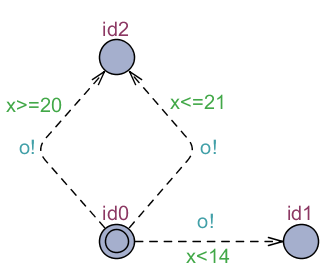
\includegraphics[scale = 0.7]{figures/determ.png}
    \caption{Non-deterministic automaton test case, which is not caught by \ecdar 0.10.}
    \label{fig:K7}
\end{figure}

\section{Consistency tests} \label{sec:consistTests}
An important part of the tests that were performed are the consistency tests. We have tried to create automata which would include the rarest corner cases. The case illustrated in Figure \ref{fig:G17}, where the consistency check starts in location \textbf{id0} satisfies the least fixpoint consistency check, but not the greatest fixpoint consistency check. It is important to remember that the least fixpoint consistency permits pruning of output edges if the property of independent progress has already been satisfied for a given location. Since the property of independent progress is satisfied already in location \textbf{id0} and there are no outgoing input edges, which are mandatory to explore, the algorithm prunes the rest of the automaton.

\begin{figure}
    \centering
    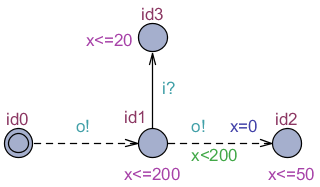
\includegraphics[scale = 0.8]{figures/test-aut-leastCons.png}
    \caption{Automaton that will only satisfy the least fixpoint consistency check.}
    \label{fig:G17}
\end{figure}

Note how the rest of the automaton does not satisfy the property of independent progress. In location \textbf{id1} the independent progress property is violated by the corresponding invariant ($x\leq200$) which disallows delaying indefinitely. Moreover, both outgoing edges from location \textbf{id1} must then be explored. Since the targets of those edges cannot ensure independent progress either, we conclude that none of the three mentioned locations would satisfy the consistency check. With that being said, this test case automaton can only satisfy the least fixpoint consistency check due to pruning of the rest of the automaton, except for location \textbf{id0}.


\section{Implementation tests}
The defining property of the implementation check is the one of the output urgency. It requires any output edge to be traversable only with a single clock valuation, without the possibility to delay instead. Consider the test case illustrated in Figure \ref{fig:G19}. This automaton is consistent and the only output edge it has is urgent, which satisfies the property of the output urgency for the entire automaton. 

Moreover, it is important to remember that the implementation check also requires a consistency check that is different from the least fixpoint consistency check mentioned previously in this chapter. Since the property of output urgency concerns all output edges, the corresponding consistency check should not be allowed to prune these edges, resulting in having to perform a full consistency check, which was described in Section \ref{sec:minConsistency}. Thus, having an invariant on location with \textbf{id2} makes the implementation check fail due to the property of independent progress not being satisfied.
\begin{figure}
    \centering
    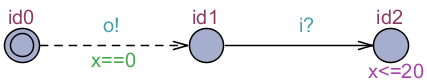
\includegraphics[scale = 0.7]{figures/G19.png}
    \caption{Automaton that fails full consistency check that is required by implementation check.}
    \label{fig:G19}
\end{figure}

\section{Summary}

To conclude the chapter, more thorough and detailed testing was done for all the existing and newly implemented features. In particular, we focused on testing all the corner cases that were discovered during this project as well as cases where \ecdar 0.10 has shown to be inconsistent with the theory.

In total there are currently more than 330 quality tests in \jecdar, which is 170 more than in the previous version of the engine. The code coverage of the most vital functionality related to feature verification has also been improved from previously achieved more than 95 percent to a complete 100 percent coverage, as can be seen in Figure \ref{fig:code-coverage}. What is more important, in its implementation \jecdar does not contain the same inconsistencies with the theory as discovered in \ecdar 0.10.

\begin{figure}
    \centering
    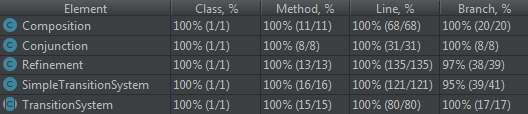
\includegraphics[scale = 0.7]{figures/code-coverage.png}
    \caption{Code and branch coverage of the most important verification algorithms.}
    \label{fig:code-coverage}
\end{figure}

In addition to the line coverage metrics, we have also considered branch coverage. It measures if all decision outcomes have been tested, where a decision can be \textit{if} and \textit{case} statements, \textit{while} and \textit{for} loops. This metrics shows if all branches (possible cases of decisions) were ever reached and consequently if the test case suite covers all possible decisions. 

The current test case suite of \jecdar achieves a minimum of 95 percent branch coverage (Figure \ref{fig:code-coverage}). The missing percentage of the branch coverage for \textit{Refinement} and \textit{SimpleTransitionSystem} classes is related to checking validity of the DBM zone, which appears to never be invalid and thus does not explore the negative outcome of an IF statement. However, such cases do not influence the correctness of the algorithms as they are validity checks that appear to never fail. Therefore we deem it not important.